\section{Robottens højde}
\label{sec:RHeight}
%
I dette afsnit analyseres resultaterne med udgangspunkt i de fem forskellige højder robotten havde i testen. For hver højde er der mellem 7-10 testpersoner. De forskellige højder fremgår af \autoref{tab:RHeight}, hvor antallet af testpersoner ligeledes er opgivet. Det undersøges hvordan robottens højde påvirker de rejsendes oplevelse af robotten, ved at undersøge hvordan resultaterne ændrer sig afhængigt af de fem forskellige højder. Det er \textit{Between-subject} design, da hver testperson kun har oplevet robotten i én af højderne og svaret ud fra denne.
%
\begin{table}[H]
\centering
\begin{tabular}{c|c}
Højde (cm) & Antal testpersoner \\ \hline
118   & 9     \\ \hline
123.5 & 10    \\ \hline
129   & 9     \\ \hline
140   & 7     \\ \hline
151   & 8    \\
\end{tabular}
\caption{Oversigt over antallet af testpersoner til hver af de fem højde robotten havde.}
\label{tab:RHeight}
\end{table}
\noindent
%
Ud fra \textit{Scree}-plottet på \autoref{fig:RHeight-Scree} fremgår det at cirka 80 \& af variansen kan forklares ud fra de to første \textit{Principal Components} (PC). Ved at tage PC3 med, opnåes cirka 94 \% forklaret varians. Det er dog væsentligt simplere, at fortolke resultaterne i to dimensioner og der fokuseres derfor som udgangspunkt kun på de to primære komponenter.
%
\begin{figure}[H]
\centering
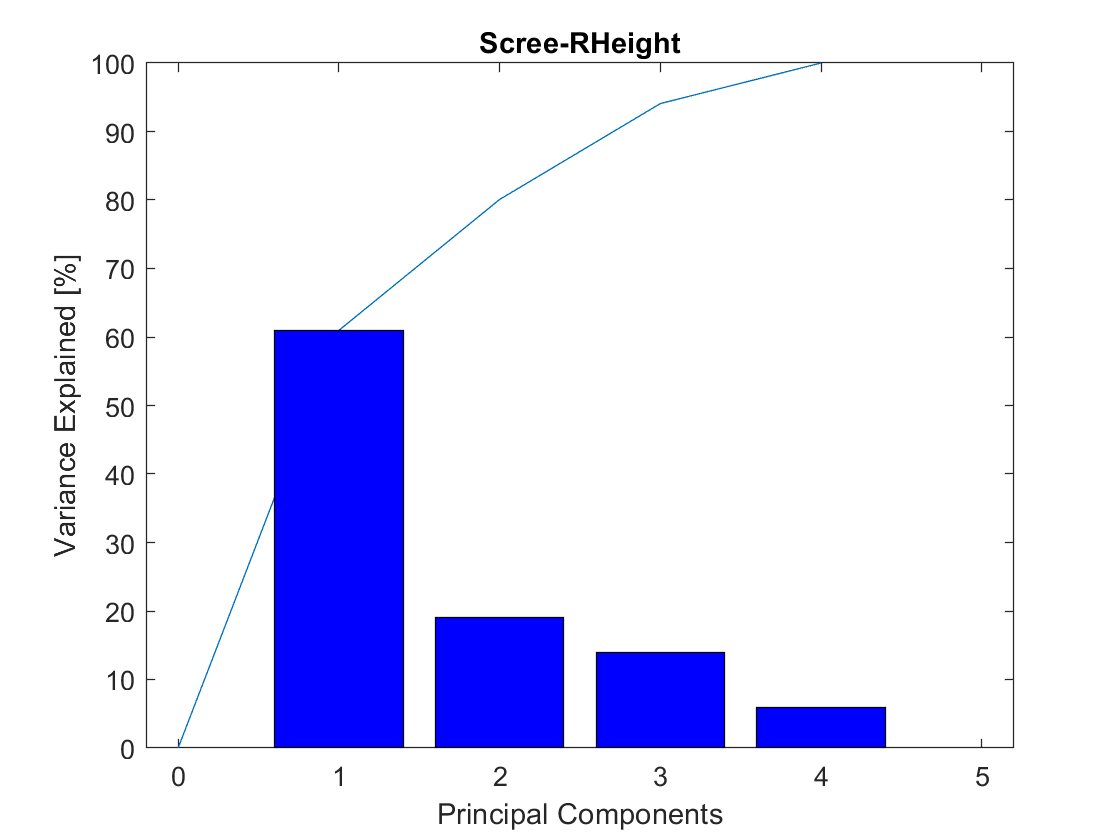
\includegraphics[width=\textwidth]{Figure/DatabehandlingSkalaer/PCAfigures/RHeight-Scree.png}
\caption{\textit{Scree}-plot, hvorpå sammenhængen mellem antallet af \textit{Principal Components} og \textit{Variance Explained [\%]} fremgår.}
\label{fig:RHeight-Scree}
\end{figure}
\noindent
%
Ud fra \textit{Score}-plottet på \autoref{fig:RHeight-Score} fremgår det, at der generelt er en del spredning mellem resultaterne ud fra de fem forskellige højder, men at 129 cm og 140 cm har lignende karakteristikker, da de ligger meget tæt i plottet.
%
\begin{figure}[H]
\centering
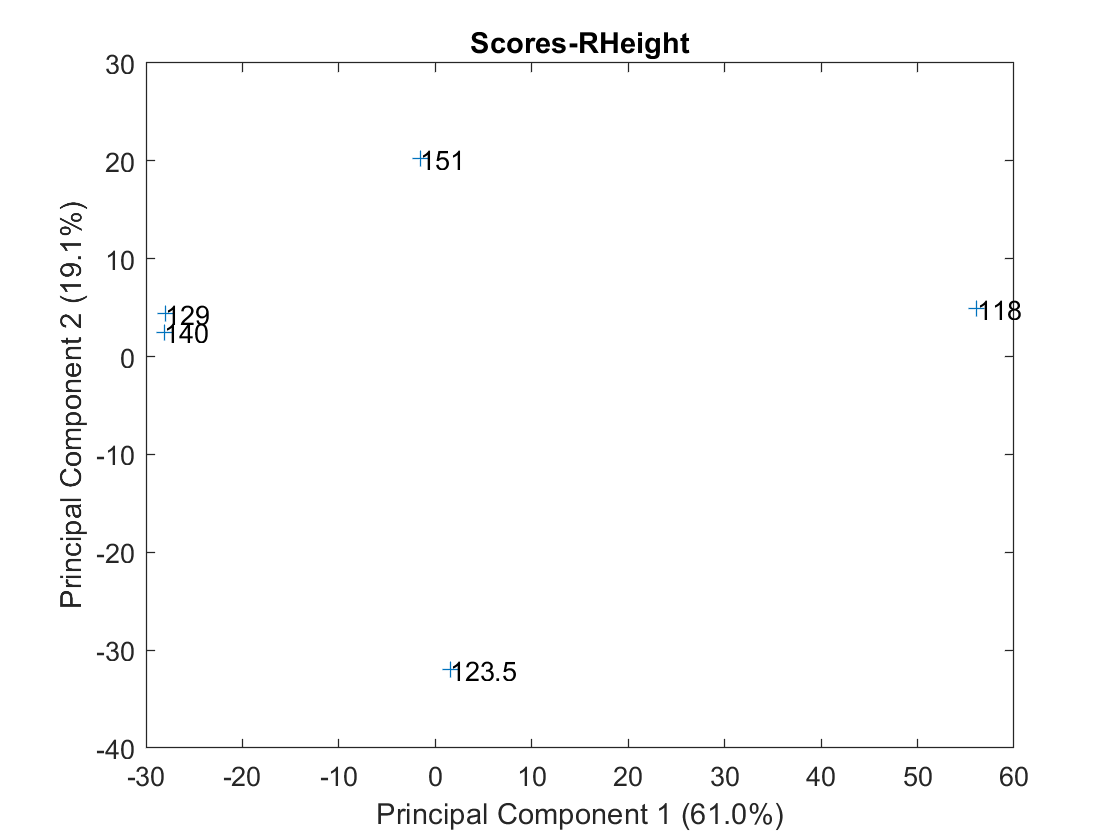
\includegraphics[width=\textwidth]{Figure/DatabehandlingSkalaer/PCAfigures/RHeight-Scores}
\caption{\textit{Score}-plot for PC1 og PC2 i forhold til robottens højde.}
\label{fig:RHeight-Score}
\end{figure}
\noindent
%
Ud fra \textit{Bi}-plottet på \autoref{fig:RHeight-Biplot}, hvorpå \textit{loadings} og \textit{scores} for hver parameter er præsenteret, fremgår det at SQ19 bidrager mest til PC1, SQ1 bidrager mest til PC2 og at SQ5, SQ7, SQ11 og SQ14 forklarer en meget lille del af variansen, hvorfor det ikke giver mening at kommentere på hvordan de indbyrdes ligger. Når to eller flere parametre ligger tæt på hinanden, er det et udtryk for, at de er højest korrelerede. Dette gør sig gældende for SQ2 og SQ4, som henholdvis dækker over hvordan testpersonerne oplevede robotten i forhold til om det er ekstremt afvisende eller ekstremt imødekommende, og hvordan robottens bevægelser blev oplevet i forhold til om bevægelserne er ekstremt rolige eller ekstremt vilde. Lignende er gældende for SQ12 og SQ18, som henholdvist dækker over hvorvidt testpersonerne kan lide at blive betjent af robotten og om de synes at robotten er spændende. SQ14 og SQ15 tyder også på at korrelere, da de nærmest ligger oven på hinanden, de to parametre vedrører henholdvist hvor personlig robottens hjælp opleves og hvor overrasket testpersonen blev over robottens henvendelse. Lignende er gældende for SQ8 og SQ17, som også ligger relativt tæt, de to parametre vedrører henholdvist hvorhvidt testpersonerne føler at robotten kan hjælpe en og hvor elegant robotten er. 

Derudover forekommer det at SQ21 er negativt korrelerede med både SQ12 og SQ18, hvor SQ21 vedrører hvor anmassende robotten robotten opleves. SQ9 er negativt korreleret med både SQ2 og SQ4, som er højt korrelerede, hvor SQ9 vedrører hvorvidt robotten stod i vejen. Derudover forekommer der også negativ korrelation mellem SQ16, som vedrører hvor irriterende robotten er, og SQ19, som vedrører hvor sød robotten er. Ydermere forekommer der en negativ korrelation mellem SQ3, som vedrører hvor nemt det var at bruge robotten, og SQ23, som vedrører hvor menneskelig robotten oplevels.  

I henhold til robottens højde, så ligger 118 cm i modsatte ende af PC1 i forhold til både 129 cm og 140 cm, som nærmest ligger oveni hinanden. Baseret på \autoref{fig:RHeight-Biplot} tyder det derfor på at højderne 129 cm og 140 cm primært er domineret af SQ21, som vedrører hvor anmassende robotten opleves, og delvist af SQ16, som vedrører hvor irriterende robotten opleves, og SQ9, som vedrører hvorvidt robotten stod i vejen. For højde 118 cm tyder det derimod på, at den højde er domineret af SQ8, som vedrører hvorvidt testpersonen føler at robotten kan hjælpe en, og delvist af SQ19, som vedrører hvor sød robotten opleves, og SQ12, som vedrører hvor godt testpersonen kan lide at blive betjent af robotten. 

Lignede gør sig gældende for PC2, hvor højderne 123.5 cm og 151 cm adskiller sig. Baseret på \autoref{fig:RHeight-Biplot} fremgår det at SQ23, som vedrører hvor menneskelig robotten opleves, primært dominerer denne højde. Dertil domineres højden også af SQ13, som vedrører hvorvidt testpersonen regnede med at robotten fulgte dem hen til det sted de havde valgt. Højden på 151 cm er derimod primært domineret af SQ3, som vedrører hvor nemt det var at bruge robotten, samt SQ1, som vedrører skærmens reaktion. 
%
\begin{figure}[H]
\centering
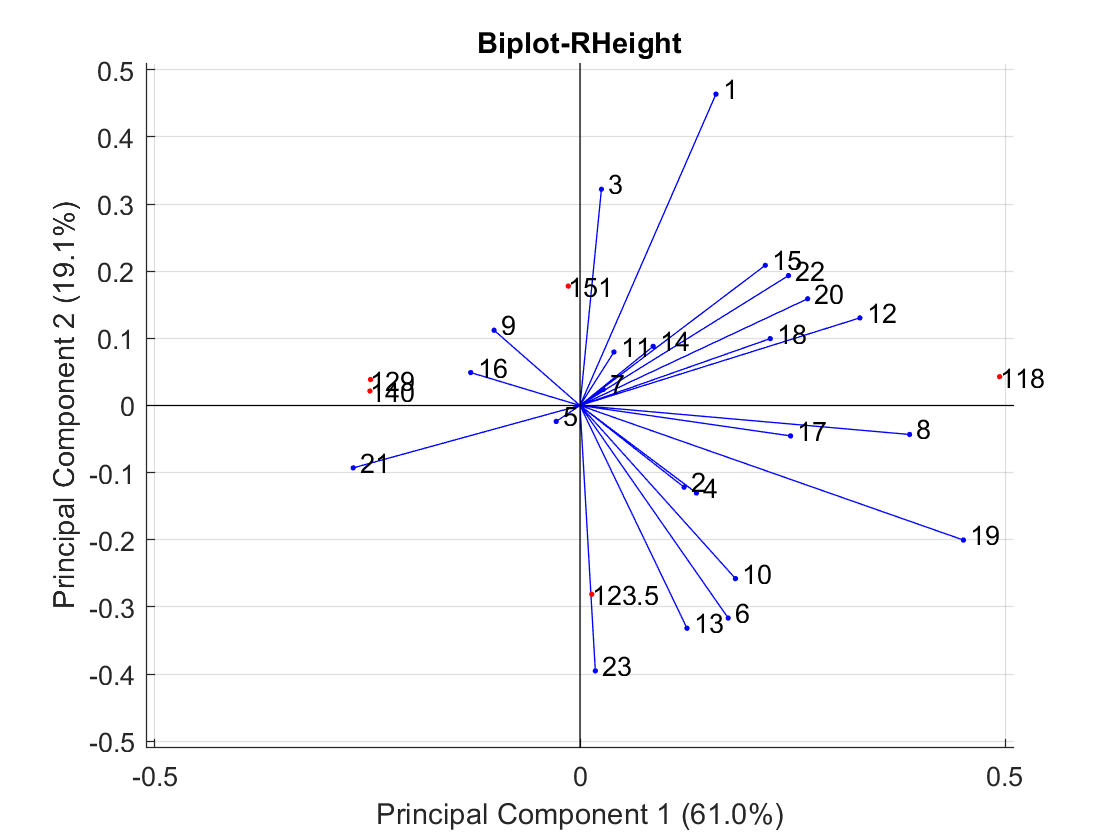
\includegraphics[width=\textwidth]{Figure/DatabehandlingSkalaer/PCAfigures/RHeight-Biplot.png}
\caption{\textit{Bi}-plot med både \textit{loadings} (angivet med blå) og \textit{scores} (angivet med rød) fremgår i forhold til robottens højde.}
\label{fig:RHeight-Biplot}
\end{figure}
\noindent
%
 Ud fra loadings i tabel XX kan det ses at ... bidrager til...

S


Tages der derimod udgangspunkt i et tredimensionelt \textit{Bi}-plot, jævnfør \autoref{fig:RHeight-3D}, fremgår det, at de to højder: 129 cm og 140 cm adskiller sig en del i den tredje dimension. Derudover tyder det på at SQ6, som vedrører testpersonernes oplevelse af robottens hastighed, samt SQ10, som vedrører hvor tryg testpersonen følte sig ved robotten, er de to parametre, som har størst indflydelse på PC3. 

Derudover elimineres nogen af de førnævnte korrelationer mellem parametrene, når de præsenteres i det tredimensionelle plot, gengivet på \autoref{fig:RHeight-3D}. Dette gælder blandt andet SQ2 og SQ4, som ikke længere ligger oven på hinanden.   
%
\begin{figure}[H]
\centering
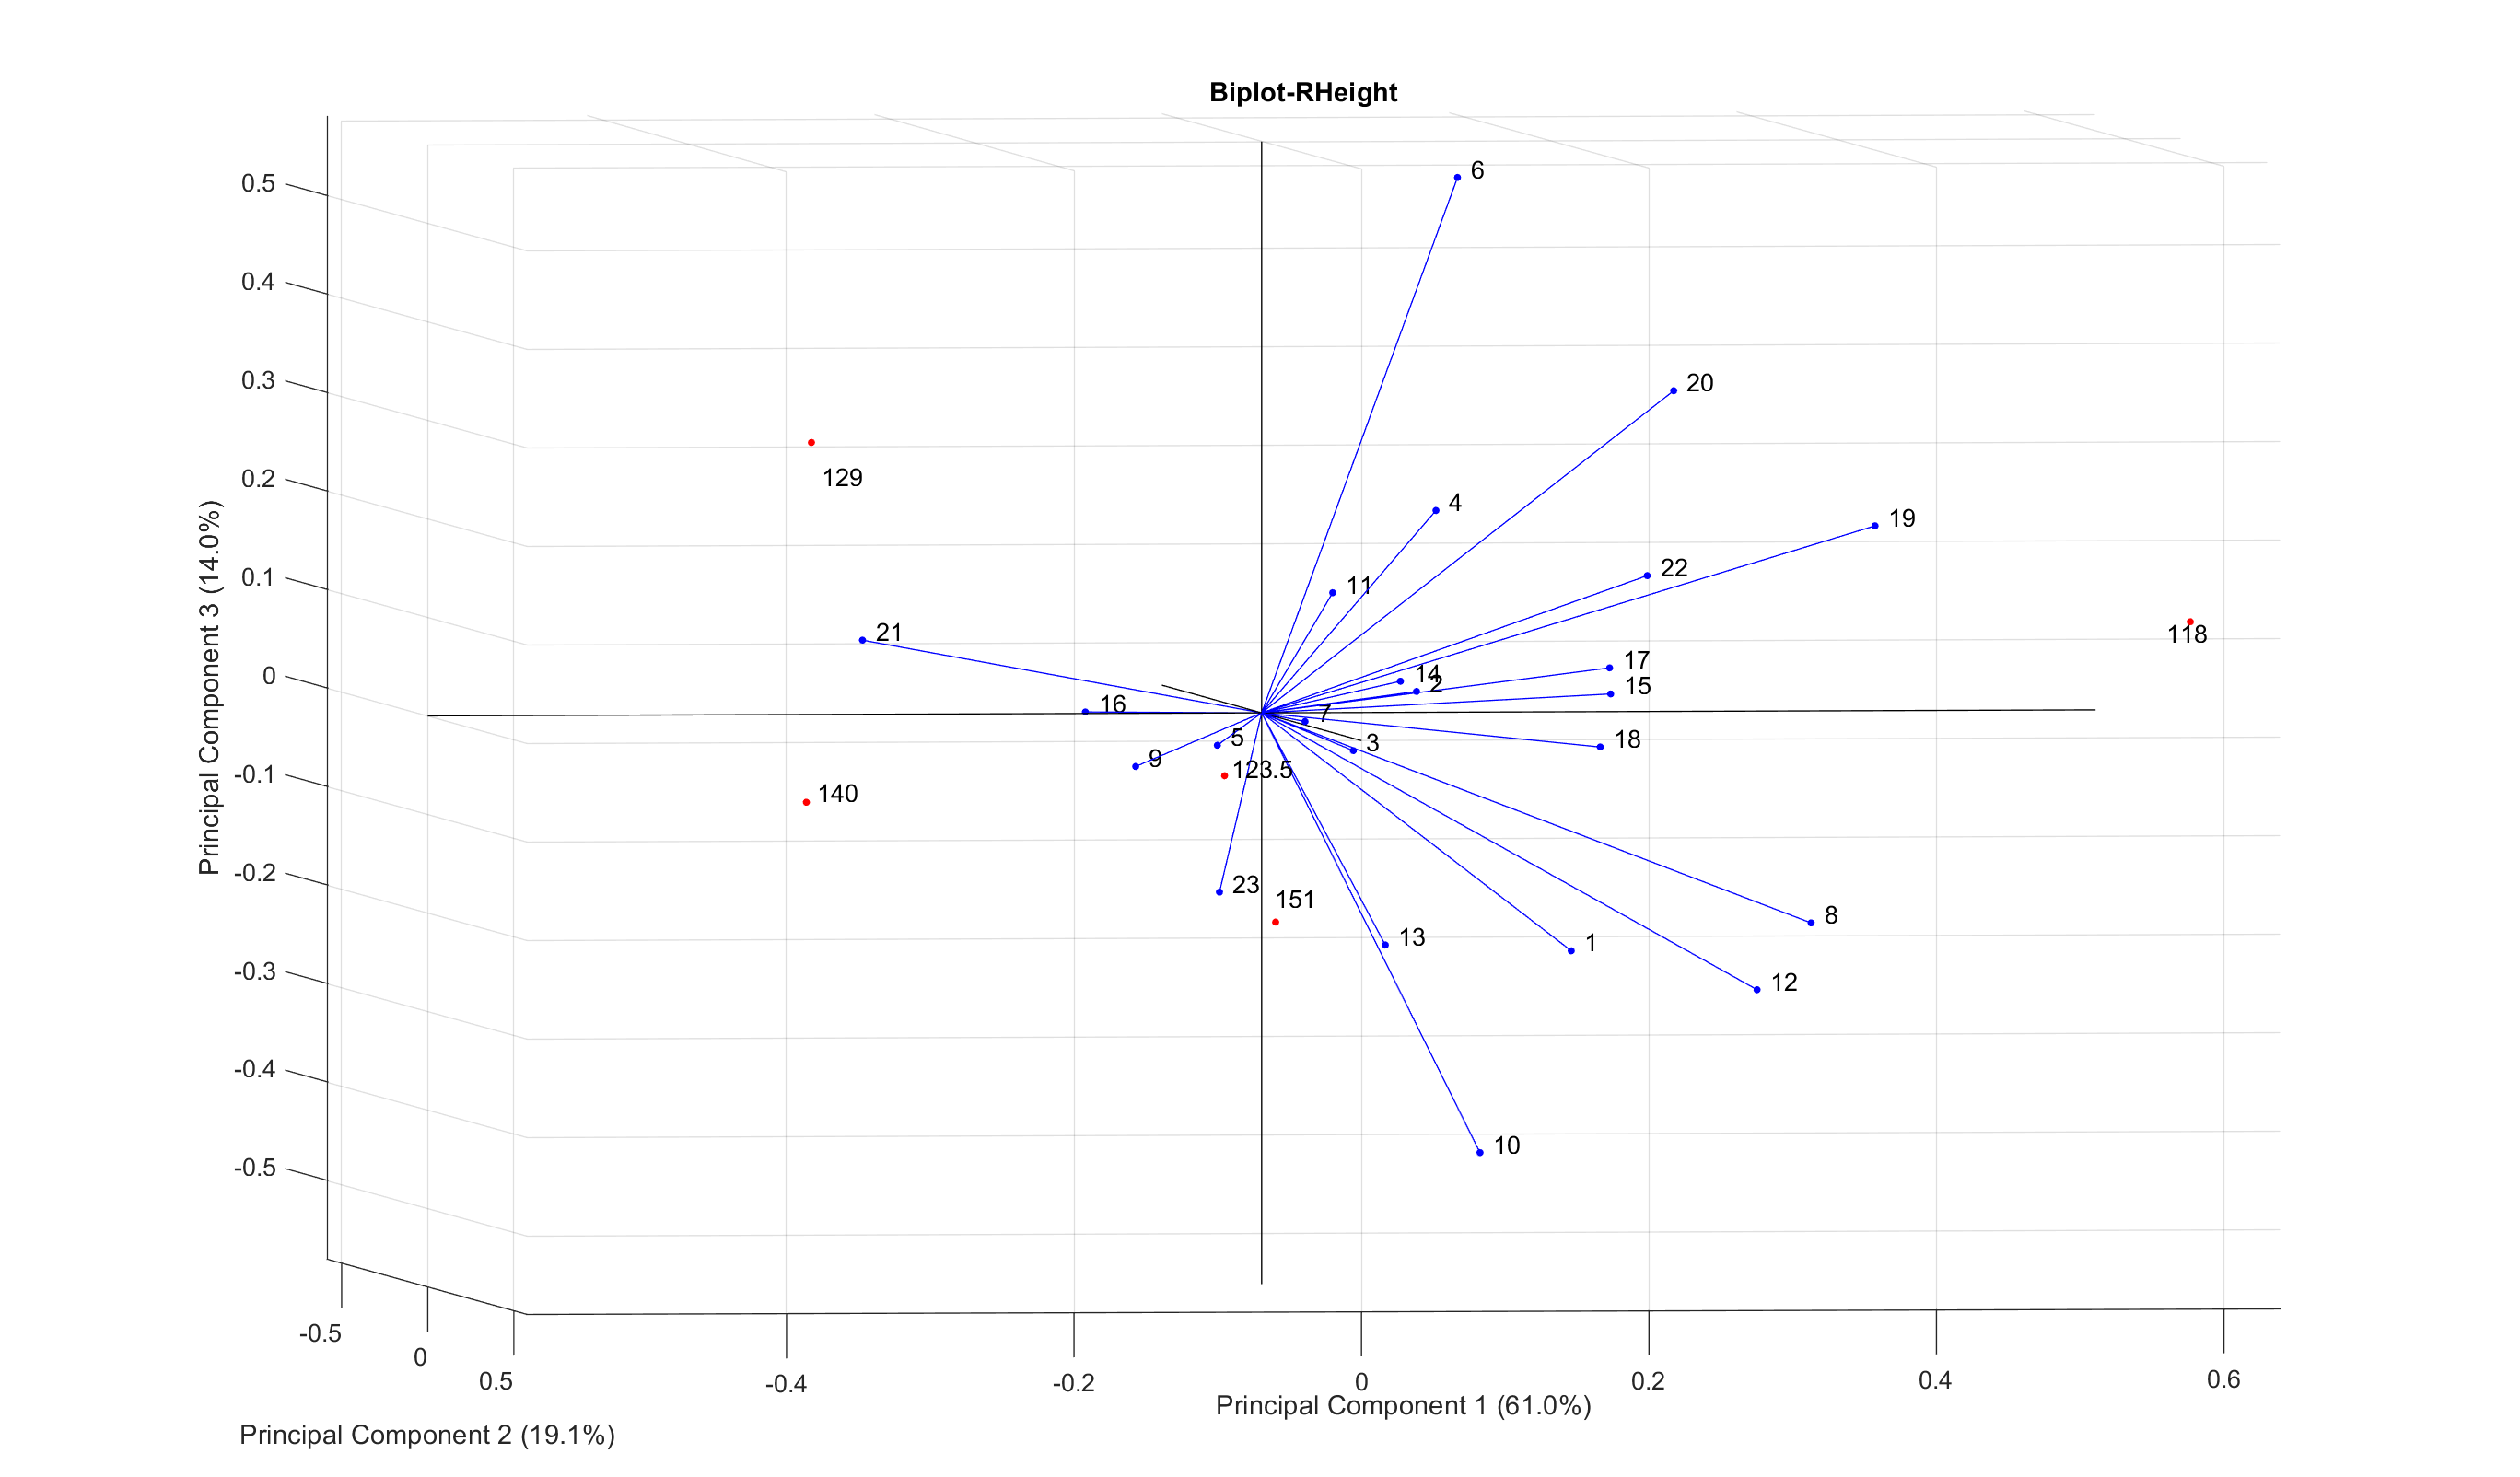
\includegraphics[width=\textwidth]{Figure/DatabehandlingSkalaer/PCAfigures/RHeight-3D.png}
\caption{3D \textit{Bi}-plot med både \textit{loadings} (angivet med blå) og \textit{scores} (angivet med rød) fremgår i forhold til robottens højde.}
\label{fig:RHeight-3D}
\end{figure}